\documentclass{article}
\usepackage{graphicx} % Required for inserting images
\usepackage{amsmath}
\usepackage{amssymb}
\usepackage{amsfonts}
\usepackage{verbatim}
\usepackage{stmaryrd}
%\usepackage{bussproofs}
\usepackage{mathabx}
\usepackage{color}
\usepackage{tikz}
\usetikzlibrary {automata,positioning}

\newcommand{\setenc}[1]{\llparenthesis #1 \rrparenthesis}
\newcommand{\set}[1]{\{#1\}}
\newcommand{\tuple}[1]{\langle #1\rangle}
\newcommand{\true}{\texttt{true}}
\newcommand{\false}{\texttt{false}}
\renewcommand{\diamond}{\lozenge} %%\diamondsuit
\newcommand{\Next}{\ovoid} %{\circ}
\newcommand{\Nat}{\mathbb{N}}
\newcommand{\sem}[1]{\llbracket #1\rrbracket}
\newtheorem{property}{Property.}


% title of this article/assignment
\title{COSC437 Security Protocols: Assignment 1}
\author{Name: Navaneethakrishna Sridhar \\ Student ID: 12590145}
\date{16 Aug 2026}

\begin{document}

\maketitle

\paragraph{Question 1. ($2$ marks)}
Create a TLA+ model that works in the same way as the Beverage machine given in the slides of week $3$'s lecture, where the transition actions are labels on the edges, and state variables (of boolean type) are (coloured) labels on the states. 
Recall that an TLA+ model is usually defined by the following predicate:
\begin{verbatim}
Spec == Init /\ [][Next]_vars    
\end{verbatim}
where $\texttt{vars}$ is the vector of state variables, and the $\texttt{[Next]\_vars}$ notation allows the system to stutter, i.e., for all reachable states $s$, $s\rightarrow s$ is always possible by $s$ making a self-transition. (We do \emph{not} assume \emph{fairness} in this question. Fairness asserts that for some action $a$, if $a$ is enabled from a state $s$ and $s$ is visited infinitely often, then $a$ must be performed infinitely often. Fairness may be required in your next assignment.)

Specify the following LTL property and verify it for your model in the TLA+ toolbox, and briefly explain the model checking result from the toolbox. Submit a ``.tla" file which contains the model and the specification predicate.

\begin{property}
In all reachable states $s$, if $pay = \texttt{TRUE}$, then sometime in the future, we must reach a state where $coke = \texttt{TRUE}$.    
\end{property}

\paragraph{Answer.}
I put the model in \texttt{Beverage.tla}. The week~3 machine has four states (\texttt{pay}, \texttt{select}, \texttt{coke}, \texttt{sprite}), so I used four boolean variables and made sure exactly one of them is \texttt{TRUE} at a time. The actions are just the edge labels: \texttt{InsertCoin} takes you from $pay$ to $select$, \texttt{TauCoke}/\texttt{TauSprite} go from $select$ to a drink, and \texttt{GetCoke}/\texttt{GetSprite} go back to $pay$. There is no fairness, as the question said:
\begin{verbatim}
Spec == Init /\ [][Next]_vars
PayLeadsToCoke == [](pay => <>coke)
\end{verbatim}
That is the LTL property $\Box(pay \rightarrow \diamond coke)$: whenever we are in $pay$, we should eventually reach $coke$.

TLC says \texttt{PayLeadsToCoke} is \emph{violated}. The error trace it gave me was:
\begin{center}
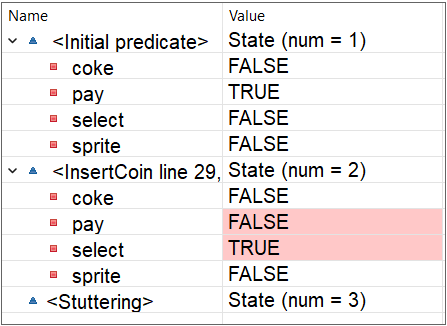
\includegraphics[width=0.75\textwidth]{images/Q1 TLC.png}
\end{center}
We start in $pay$, so $\diamond coke$ has to hold on this path, but $coke$ never becomes true. The last step is labelled \texttt{Stuttering}. That is not deadlock (\texttt{TauCoke} is still enabled from $select$) it just means the machine can sit there doing nothing. \texttt{[][Next]\_vars} always allows a self-loop that leaves the variables unchanged, and since I did not add $WF$/$SF$, TLC is allowed to take that loop forever. (It would also fail if the machine always chose sprite and never coke.)

\bigskip \bigskip

\paragraph{Question 2. ($2$ marks)}
We refer to the TLA+ model ``\texttt{Peterson.tla}" posted in the Learn page. You will need to initialize the variable \texttt{Procs} with the set $\set{0, 1}$ before running a model checking algorithm in a model. \textit{(If you do not remember how to do it, check the course recording.)} Assuming the two processes are denoted $0$ and $1$, write down the following properties and verify them in the TLA+ toolbox. Briefly explain the results produced by model checking.

\begin{enumerate}
    \item In all reachable states $s$, if $pc[0]=``ncs"$ in $s$, then sometime in the future the system must enter a state where $pc[0]=``cs"$.
    \item In all reachable states $s$, if $pc[0]=``ncs"$ in $s$, then sometime in the future the system must enter a state where $pc[0]=``e4"$.
\end{enumerate}

\paragraph{Answer.}
I set $\texttt{Procs}=\set{0,1}$ in the Toolbox and checked these one at a time:
\begin{verbatim}
NcsToCs == [](pc[0] = "ncs" => <>(pc[0] = "cs"))
NcsToE4 == [](pc[0] = "ncs" => <>(pc[0] = "e4"))
\end{verbatim}
\texttt{Spec} already includes $\texttt{SF\_vars(P(0))}\wedge\texttt{SF\_vars(P(1))}$. \texttt{e4} is the backoff branch of the entry protocol, not the exit from $cs$ (that is \texttt{exit}/\texttt{x2}).

\textbf{(i)} TLC reported \emph{no error} for \texttt{NcsToCs} (190 distinct states). Fairness applies to the whole process, so process~$0$ cannot stay in $ncs$ forever and then has to reach $cs$.

\textbf{(ii)} TLC reported that \texttt{NcsToE4} is \emph{violated}. The trace is a fair loop (\texttt{Back to state 2}): process~$0$ keeps taking the uncontended $e2$ branch ($\texttt{flag}[1]=\texttt{FALSE}$ goes straight to $cs$) and never visits $e4$.

\bigskip \bigskip

\paragraph{Question 3. ($3$ marks)} Consider the following temporal logic formulas that are claimed to be equivalent, assuming $p, p_1, p_2, p_3, q\in AP$:

\begin{itemize}
    \item[$LTL$] formulas:\\ \textbf{(a)} $\diamond\ \Box\ p\equiv\Box\ \diamond\ p$, \\
    \textbf{(b)} $\neg\Box\ p\equiv\diamond\neg p$, \\
    \textbf{(c)} $\Box\ (p\rightarrow\ \diamond\ q) \equiv \diamond\ (p\rightarrow\ \Box\ q)$, \\
    \textbf{(d)} $\Box\ (p_1\vee p_2)\equiv (\Box\ p_1)\vee(\Box\ p_2)$, \\
    \textbf{(e)} $\diamond\ p\equiv p\vee(\Next\ \diamond\ p)$, \\
    \textbf{(f)} $p_1\ U\ (p_2\vee p_3)\equiv(p_1\ U\ p_2)\vee(p_1\ U\ p_3)$; 
    \item[$CTL$] formulas: \\
    \textbf{(g)} $AF\ AG\ p\equiv AG\ AF\ p$, \\
    \textbf{(h)} $AG\ (p_1\vee p_2) \equiv (AG\ p_1)\vee(AG\ p_2)$, \\
    \textbf{(i)} $AF\ (p_1\wedge p_2) \equiv (AF\ p_1)\wedge(AF\ p_2)$, \\
    \textbf{(j)} $EF\ p\vee EF\ q\equiv EF\ (p\vee q)$,\\
    \textbf{(k)} $p\ AU\ (EX\ q)\equiv EX (p\ AU\ q)$\\
    \textbf{(l)} $p_1\ EU\ p_2\equiv (p_1\vee p_2)\ EU\ p_2$.
\end{itemize}

\bigskip

For each pair of formulas \textbf{(b)-(f)} and \textbf{(h)-(l)}, answer whether the equivalence (represented by ``$\equiv$'') is $\true$ or $\false$. If you think an item is $\true$, you only need to explain why it is the case by using no more than two sentences. If an item is $\false$, draw a simple transition system (for CTL) or an infinite path (for LTL) that indicates the difference (i.e., the system you draw should be a model that satisfies one formula but not the other). You may draw the states and transitions by hand and then scan the paper, or use a drawing software to generate a picture (insert with \texttt{graphicx}), or use the latex drawing packages such as \texttt{PSTricks} and \texttt{TikZ/PGF}. A scanned hand-drawing is acceptable only if it is readable.

As an example, we know that \textbf{(a)} is false. The following infinite path has $p$ hold in every odd state. In the same path, every even state does not have $p$ as they are not labelled with any proposition in $AP$. This infinite path satisfies $\Box\ \diamond\ p$ but does not satisfy $\diamond\ \Box\ p$, as the property $\diamond\ \Box\ p$ requires a trace to have $p$ hold forever after reaching a future state.

\bigskip

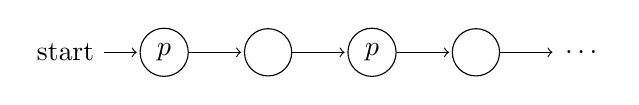
\begin{tikzpicture}[shorten >=1pt,node distance=0.7cm,auto,every state/.style={minimum size=0.6cm}]
    \node[state, initial] (q0) {$p$};
    \node[state] (q1) [right=of q0] {};
    \node[state] (q2) [right=of q1] {$p$};
    \node[state] (q3) [right=of q2] {};
    \node (q4) [right=of q3] {$\dots$};
    \path[->] (q0) edge (q1);
    \path[->] (q1) edge (q2); 
    \path[->] (q2) edge (q3);
    \path[->] (q3) edge (q4); 
\end{tikzpicture}


\bigskip

\textbf{(g)} is also false. The initial state of the following finite-state system does not satisfy $AF\ AG\ p$. But it satisfies $AG\ AF\ p$. In fact, unfolding this transition system yields an infinite trace that is the same as the above example.

\bigskip

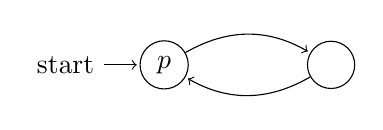
\begin{tikzpicture}[shorten >=1pt,node distance=1.5cm,auto,every state/.style={minimum size=0.6cm}]
    \node[state, initial] (q0) {$p$};
    \node[state] (q1) [right=of q0] {};
    \path[->] (q0) edge[bend left] (q1);
    \path[->] (q1) edge[bend left] (q0); 
\end{tikzpicture}

\paragraph{Answer.}
We use the week-4 definitions: LTL equivalence means the two formulas hold of exactly the same infinite paths; CTL equivalence means they have the same satisfying states.

\medskip
\textbf{(b)} $\true$. This is the De~Morgan dual of $\Box$: $\neg\diamond\phi\equiv\Box\neg\phi$, and swapping $\phi$ for $\neg p$ gives $\neg\Box p\equiv\diamond\neg p$.

\medskip
\textbf{(c)} $\false$. On the path below, $\Box(p\rightarrow\diamond q)$ fails because we start in $p$ and $q$ never appears. $\diamond(p\rightarrow\Box q)$ still holds since $\diamond$ only needs the implication at \emph{some} state, and from the second state $p$ is false, so $p\rightarrow\Box q$ is true even though $q$ never occurs.

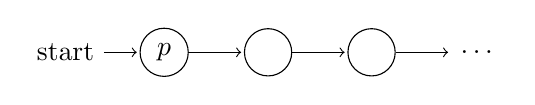
\begin{tikzpicture}[shorten >=1pt,node distance=0.7cm,auto,every state/.style={minimum size=0.6cm}]
    \node[state, initial] (q0) {$p$};
    \node[state] (q1) [right=of q0] {};
    \node[state] (q2) [right=of q1] {};
    \node (q3) [right=of q2] {$\dots$};
    \path[->] (q0) edge (q1);
    \path[->] (q1) edge (q2);
    \path[->] (q2) edge (q3);
\end{tikzpicture}

\medskip
\textbf{(d)} $\false$. Same idea as (a), but alternating $p_1$ and $p_2$. Every state has $p_1$ or $p_2$, so $\Box(p_1\vee p_2)$ holds, but neither proposition holds forever.

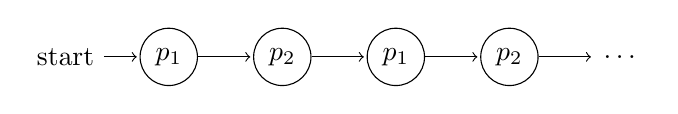
\begin{tikzpicture}[shorten >=1pt,node distance=0.7cm,auto,every state/.style={minimum size=0.6cm}]
    \node[state, initial] (q0) {$p_1$};
    \node[state] (q1) [right=of q0] {$p_2$};
    \node[state] (q2) [right=of q1] {$p_1$};
    \node[state] (q3) [right=of q2] {$p_2$};
    \node (q4) [right=of q3] {$\dots$};
    \path[->] (q0) edge (q1);
    \path[->] (q1) edge (q2);
    \path[->] (q2) edge (q3);
    \path[->] (q3) edge (q4);
\end{tikzpicture}

\medskip
\textbf{(e)} $\true$. $\diamond p$ is $\mathrm{true}\,U\,p$, and unfolding until gives $p$ now or $\diamond p$ in the next state, i.e.\ $p\vee(\Next\diamond p)$.

\medskip
\textbf{(f)} $\true$. If $p_1\,U\,(p_2\vee p_3)$ holds, there is a first time $p_2$ or $p_3$ is true, and $p_1$ holds until then. Thus, $p_1\,U\,p_2$ or $p_1\,U\,p_3$ holds.

\medskip
\textbf{(h)} $\false$. Every reachable state has $p_1$ or $p_2$, so $AG(p_1\vee p_2)$ holds at the start, but neither $AG p_1$ nor $AG p_2$ does, because we keep switching.

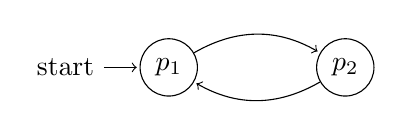
\begin{tikzpicture}[shorten >=1pt,node distance=1.5cm,auto,every state/.style={minimum size=0.6cm}]
    \node[state, initial] (q0) {$p_1$};
    \node[state] (q1) [right=of q0] {$p_2$};
    \path[->] (q0) edge[bend left] (q1);
    \path[->] (q1) edge[bend left] (q0);
\end{tikzpicture}

\medskip
\textbf{(i)} $\false$. The only path eventually hits $p_1$ and later hits $p_2$, so $(AF p_1)\wedge(AF p_2)$ holds because they do not have to be true in the same state. $AF(p_1\wedge p_2)$ fails because no state is labelled with both.

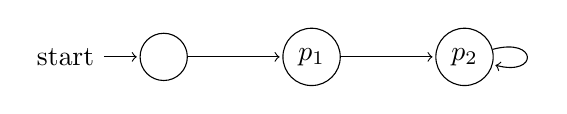
\begin{tikzpicture}[shorten >=1pt,node distance=1.2cm,auto,every state/.style={minimum size=0.6cm}]
    \node[state, initial] (q0) {};
    \node[state] (q1) [right=of q0] {$p_1$};
    \node[state] (q2) [right=of q1] {$p_2$};
    \path[->] (q0) edge (q1);
    \path[->] (q1) edge (q2);
    \path[->] (q2) edge[loop right] (q2);
\end{tikzpicture}

\medskip
\textbf{(j)} $\true$. $EF\phi$ just means a $\phi$-state is reachable, so being able to reach $p$ or reach $q$ is the same as being able to reach a state labelled $p\vee q$.

\medskip
\textbf{(k)} $\false$. From the start, $p$ holds until the middle state, and that middle state has a $q$-successor, so $p\,AU\,(EX q)$ holds. $EX(p\,AU\,q)$ fails because the only next state has neither $p$ nor $q$.

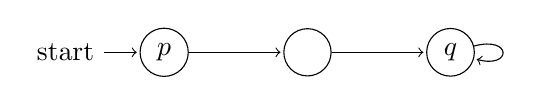
\begin{tikzpicture}[shorten >=1pt,node distance=1.2cm,auto,every state/.style={minimum size=0.6cm}]
    \node[state, initial] (q0) {$p$};
    \node[state] (q1) [right=of q0] {};
    \node[state] (q2) [right=of q1] {$q$};
    \path[->] (q0) edge (q1);
    \path[->] (q1) edge (q2);
    \path[->] (q2) edge[loop right] (q2);
\end{tikzpicture}

\medskip
\textbf{(l)} $\true$. If $p_1\,EU\,p_2$ holds then so does $(p_1\vee p_2)\,EU\,p_2$. The other way is to take the shortest path to $p_2$, but before that, $p_2$ is false, so $p_1\vee p_2$ is just $p_1$.

\newpage

\paragraph{Question 4. ($3$ marks)} Consider the following (unlabelled) transition system with the state space
$S = \set{s_0, s_1, s_2, s_3, s_4, s_5, s_6, s_7}$, $AP = \set{a, b, c}$,
and the labelling function shown in the picture. %The action set is irrelevant to the answer of this question, therefore, the transitions are unlabelled.

\bigskip
% \fbox{picture omitted}
\begin{center}
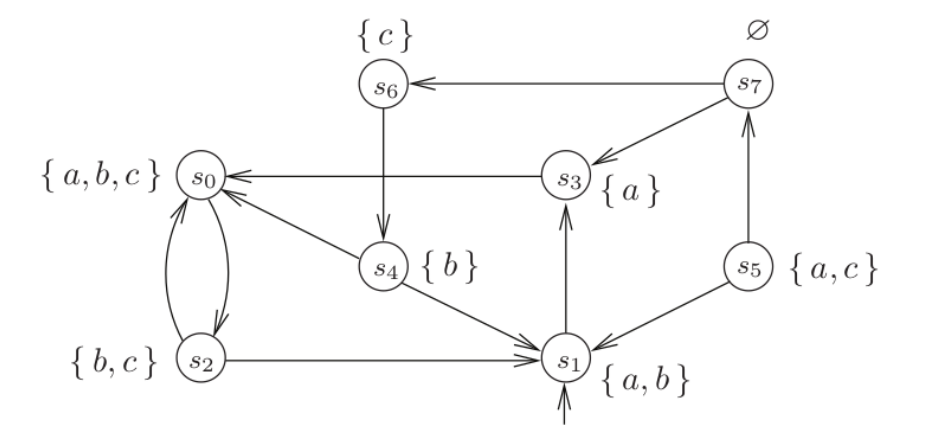
\includegraphics[width=0.75\textwidth]{images/Q4 Diagram.png}
\end{center}

\bigskip

For each of the following CTL formulas, find the set of states that satisfy the formula by running the model checking algorithms for CTL (discussed in the slides of week $4$):
\begin{itemize}
    \item[(a)] $AF\ a$
    \item[(b)] $AG\ AF\ a$
    \item[(c)] $a\ EU\ (b\wedge c)$
\end{itemize}

\paragraph{Answer.}
From the figure, $S=\set{s_0,\dots,s_7}$ and
\begin{align*}
\sem{a}&=\set{s_0,s_1,s_3,s_5},&
\sem{b}&=\set{s_0,s_1,s_2,s_4},&
\sem{c}&=\set{s_0,s_2,s_5,s_6},&
\sem{b\wedge c}&=\set{s_0,s_2}.
\end{align*}
\begin{align*}
\mathit{Post}(s_0)&=\set{s_2},&
\mathit{Post}(s_1)&=\set{s_3},&
\mathit{Post}(s_2)&=\set{s_0,s_1},&
\mathit{Post}(s_3)&=\set{s_0},\\
\mathit{Post}(s_4)&=\set{s_0,s_1},&
\mathit{Post}(s_5)&=\set{s_1,s_7},&
\mathit{Post}(s_6)&=\set{s_4},&
\mathit{Post}(s_7)&=\set{s_3,s_6}.
\end{align*}
I used the examples from the Week 4 lecture (slide 22) as a guide: start from the states that already satisfy the inner formula, then add/keep states according to their successors until the set stops changing.

\medskip
\textbf{(a)} $AF a$. Start from the $a$-states and add a state when \emph{every} successor is already in the set:
\[
\sem{AF_0 a}=\sem{a},\qquad
\sem{AF_{i+1} a}=\sem{a}\cup\set{s\mid \mathit{Post}(s)\subseteq\sem{AF_i a}}.
\]
\begin{align*}
\sem{AF_0 a}&=\set{s_0,s_1,s_3,s_5},\\
\sem{AF_1 a}&=\set{s_0,s_1,s_2,s_3,s_4,s_5}
\quad\text{($s_2\to s_0,s_1$ and $s_4\to s_0,s_1$)},\\
\sem{AF_2 a}&=\set{s_0,s_1,s_2,s_3,s_4,s_5,s_6}
\quad\text{($s_6\to s_4$)},\\
\sem{AF_3 a}&=S
\quad\text{($s_7\to s_3,s_6$)},\\
\sem{AF_4 a}&=S=\sem{AF_3 a}.
\end{align*}
So $\sem{AF a}=S=\set{s_0,s_1,s_2,s_3,s_4,s_5,s_6,s_7}$. Every path eventually hits an $a$-state.

\medskip
\textbf{(b)} $AG AF a$. Start from $\sem{AF a}$ and keep a state only if it and all of its successors stay in the set.

Every state already has a successor in $S$, so $\sem{AG_1(AF a)}=S=\sem{AG_0(AF a)}$. Thus $\sem{AG AF a}=S$.

\medskip
\textbf{(c)} $a\,EU\,(b\wedge c)$. Grow from the goal $b\wedge c$, and add an $a$-state if \emph{some} successor is already in the set:
\[
\sem{EU_0}=\sem{b\wedge c},\qquad
\sem{EU_{i+1}}=\sem{b\wedge c}\cup\bigl(\sem{a}\cap\set{s\mid \mathit{Post}(s)\cap\sem{EU_i}\neq\emptyset}\bigr).
\]
\begin{align*}
\sem{EU_0}&=\set{s_0,s_2},\\
\sem{EU_1}&=\set{s_0,s_2,s_3}
\quad\text{($s_3\to s_0$)},\\
\sem{EU_2}&=\set{s_0,s_1,s_2,s_3}
\quad\text{($s_1\to s_3$)},\\
\sem{EU_3}&=\set{s_0,s_1,s_2,s_3,s_5}
\quad\text{($s_5\to s_1$)},\\
\sem{EU_4}&=\sem{EU_3}.
\end{align*}
So $\sem{a\,EU\,(b\wedge c)}=\set{s_0,s_1,s_2,s_3,s_5}$. $s_4,s_6,s_7$ are not labelled $a$ and are not $b\wedge c$, so they never get added.

\bigskip

\bigskip

\bigskip

\paragraph{To submit your answer:} Upload a PDF file and a tla file (for Question $1$). You may either edit the tex document and then compile the file using latex/pdflatex, or by writing down your solution on a piece of paper and scan it. A scanned handwriting is acceptable only if the handwriting is readable by average humans and it is in the PDF format. Unreadable submissions will result in a $0$ mark for this assignment.


\end{document}